% !TEX TS-program = pdflatexmk
%\InputIfFileExists{a4-mancs.sty}{}{}

\documentclass[12pt,BSc,wordcount,twoside, openany, oneside]{muthesis}
\usepackage[a4paper, total={6.5in, 8in}]{geometry}
\usepackage{csquotes}

\usepackage{titlesec}
\titleformat{\chapter}[display]{\normalfont\bfseries}{}{0pt}{\Huge}

\let\subparagraph\paragraph
\let\paragraph\subsubsection
\let\subsubsection\subsection
\let\subsection\section
\let\section\chapter

\let\chaptername\relax


%% Any characters from a % to the end of line are comments.

%% The third-rep class and this starter kit were written by 
%% Graham Gough <graham@cs.man.ac.uk>
%% If you have any comments or questions regarding this document,
%% please post them to the local newsgroup man.cs.tex.

%% This skeleton report is organised as a master file called
%% report.tex which then includes files for individual parts including
%% abstract.tex, chapter1.tex, chapter2.tex, chapter3.tex and
%% appendix1.tex.  

%% The third-rep style is a locally created style based on the
%% standard LaTeX report style. If you really want to have a look at
%% it, its source can be found in
%% /usr/local/share/texmf/tex/latex/mancs/third-rep.cls
%%
%% More information about LaTeX in general and the local setup in
%% particular can be found on the web at 
%% http://csis.cs.manchester.ac.uk/software/contrib/latex
%%
%%%%%%%%%%%%%%%%%%%%%%%%%%%%%%%%%%%%%%%%%%%%%%%%%%%%%%%%%%%%%%%%%%%%%%%%
%%
%% This is an example of how you load extra packages.
%% Some packages are already loaded in the third-rep class

\usepackage{url} % typeset URL's sensibly
\usepackage[inline]{enumitem}
\onehalfspacing

\usepackage{pslatex} % Use Postscript fonts
\renewcommand{\thesection}{\arabic{section}}

\title{Extractive Summarisation of\\
  UK Annual Reports}

%% and author
\author{Vladislav Yotkov}
\stuid{10463973}
%% and supervisor
\principaladviser{Dr. Jonathan Shapiro}
%% and the year of the report
\submitdate{April 2023}

\usepackage{listings}
\usepackage{amsthm}
\newtheorem{example}{Example}
\usepackage{epigraph}
\usepackage{graphicx} % Required for inserting images
\usepackage{booktabs}
\usepackage{caption}
\usepackage{subcaption}
\usepackage{amsmath}
\usepackage{array}
\usepackage{multirow}

\usepackage{tikz}
\usetikzlibrary{shapes.geometric}
\usetikzlibrary{positioning, fit, calc, shapes, matrix, arrows.meta}
\usepackage{xcolor}
\usepackage{hyperref}
%\usepackage[colorlinks]{hyperref}
\usepackage{cite}

% page numbering
\pagenumbering{arabic}
%\usepackage{fancyhdr}
%\fancyhf{}
%\cfoot{\thepage}
%\pagestyle{fancy}

% helvetica
\fontfamily{phv}

\usepackage[acronym,toc]{glossaries}
\newglossarystyle{glossary_style}
{
    \setglossarystyle{long3colheader}%
    \renewcommand*{\glossaryheader}{}%
    \renewcommand{\glossentry}[2]{%
        \textbf{\glsentryitem{##1}\glstarget{##1}{\glossentryname{##1}}}
        & \glossentrydesc{##1}
        & ##2
        \tabularnewline}%
}

\makeglossaries
\newacronym{af}{AF}{Accounting and Finance}
\newacronym{ats}{ATS}{Automatic Text Summarisation}
\newacronym{cbow}{CBOW}{Continuous Bag of Words}
\newacronym{csf}{CSF}{Computational Shared Facility}
\newacronym{esg}{ESG}{Environmental, Social, and Governance}
\newacronym{esma}{ESMA}{European Securities and Markets Authority}
\newacronym{ets}{ETS}{Extractive Text Summarisation}
\newacronym{fcffnn}{FCFFNN}{Fully-Connected Feed-Forward Neural Network}
\newacronym{fnp}{FNP}{Financial Narrative Processing}
\newacronym{fnp21}{FNP21}{Financial Narrative Processing 2021}
\newacronym{fnp22}{FNP22}{Financial Narrative Processing 2022}
\newacronym{fns21}{FNS21}{Financial Narrative Summarisation 2021}
\newacronym{fns22}{FNS22}{Financial Narrative Summarisation 2022}
\newacronym{frc}{FRC}{Financial Reporting Council}
\newacronym{gru}{GRU}{Gated Recurrent Unit}
\newacronym{ifrs}{IFRS}{International Financial Reporting Standards}
\newacronym{lcs}{LCS}{Longest Common Subsequence}
\newacronym{lstm}{LSTM}{Long Short-Term Memory}
\newacronym{mlm}{MLM}{Masked Language Model}
\newacronym{nlp}{NLP}{Natural Language Processing}
\newacronym{ns}{NSP}{Next Sentence Prediction}
\newacronym{rouge}{ROUGE}{Recall-Oriented Understudy for Gisting Evaluation}
\newacronym{sec}{SEC}{Securities and Exchange Commission}
\newacronym{tfidf}{Tf-Idf}{Term Frequency - Inverse Document Frequency}

\begin{document}

%% This actually creates the title and abstract pages
%\dotitleandabstract
\beforeabstract

\prefacesection{Abstract}
Although there has been considerable progress in Natural Language Processing (NLP) over the years, it has not fully reached the Accounting and Finance (AF) industry.
In the meantime, companies worldwide produce vast amounts of textual data as part of their reporting packages to comply with regulations and inform shareholders of their financial performance.
The glossy annual report is such an example, widely read by investors, but it also tends to be quite long.
Inspired by the Financial Narrative Processing (FNP) workshops (\cite{zmandar-etal-2021-financial, fnp-2022-financial}),
we design an Automatic Text Summarisation (ATS) system for the narrative parts of UK financial annual reports.
With this goal in mind, we implement and explore the following models for Extractive Text Summarisation (ETS):
\begin{enumerate*}
    \item attention-based Financial Recurrent Neural Network (FinRNN) with data augmentation,
    \item fine-tuned Financial BERT (FinBERT) (\cite{yang2020finbert})
\end{enumerate*}.
Our evaluations based on the ROUGE-2 metric show both models to be outperforming the standard ATS baselines: TextRank (\cite{mihalcea-tarau-2004-textrank}), and LexRank (\cite{Erkan2004LexRankGC}).
Furthermore, our FinBERT-base model achieves a ROUGE-2 score of $0.382$ beating \emph{the best English model in the FNS22} with $0.008$ (\cite{el-haj-etal-2022-financial}).
However, we must acknowledge that these results are not official because we were not provided with the FNS22 testing data,
and we had to create our own training-validation sets, while using the official validation set as our testing one.
\afterabstract

\prefacesection{Acknowledgements}
I would like to thank my supervisor Dr. Jonathan Shapiro and Dr. Riza Batista-Navarro for the provided advice along the way. Also, this project could not have been possible without the UK annual reports data and the computing resources provided by the Financial Narrative Processing's administration and the UoM's Computational Shared Facility, respectively. 
\afterpreface

% These include the actual text
\section{Introduction}
\subsection{Financial Reports}
Due to international regulations, companies are obliged to report their periodic performance (annual, bi-annual) to various regulatory authorities\footnote{Regulation authorities worldwide:
\begin{itemize}
    \item Securities and Exchange Commission (SEC) in the USA
    \item European Securities and Markets Authority (ESMA) in Europe
    \item Financial Reporting Council (FRC) in the UK
    \item International Financial Reporting Standards (IFRS) in 167 jurisdictions worldwide
\end{itemize}
} and other users (e.g., corporate stakeholders, investors, customers, suppliers, etc.). These reports contain essential information about the operations and finances of the business, but differ in forms. For example,
\begin{enumerate}
    \item 10-K reports filed to the SEC\footnote{\url{https://www.sec.gov}} and accessible through their Electronic Data Gathering, Analysis, and Retrieval\footnote{\url{https://www.sec.gov/edgar}} (EDGAR) system. They follow a standardised template and are plain text, which makes them particularly easy for automated large-scale research (\cite{el-haj2019retrieving}). 
\end{enumerate}

As outlined in \cite{elliott1998accounting}, investors’ trust in the accountability of businesses would be based no longer as much on just the financial statements, but also on more descriptive narratives that define strategy and planning of resource use. 

\section{Background}\label{sec:background}

\subsection{Supervised Learning}\label{subsec:supervised-learning}

\subsection{TFIDF}\label{subsec:tfidf}

\subsection{Word Embeddings}\label{subsec:word-embeddings}
Historically, to represent a token (i.e., word) $w_{i}$ in a vocabulary $V$ numerically, we define a one-hot-encoding vector of all zeroes except of a one at the index of the word $w_{i}$ in $V$ (i.e., $i$).

The results are sparse individual word vectors being orthogonal to each other which \begin{enumerate*}
    \item waste memory (each word is a $|V|$-sized vector, hence a total of $|V|^{2}$ for all tokens) and more importantly
    \item fail to encode semantic similarity due to their cosine similarity being always zero
\end{enumerate*}.


Traditionally, AF research has represented an input text with the help of bag-of-words (BOW) models which can be viewed from the  \begin{enumerate*}
    \item the binary perspective - represent a whole document $d$ as a binary vector containing ones for all words $w_{i}$ occurring in $d$ from $V$, 
    \item the term frequency perspective - encode number of word occurrences in documents instead of binary representation (\cite{Xu2013AnAT}), and 
    \item the tf-idf perspective - extend the latter to penalise ubiquitous terms (\cite{SprckJones1972ASI}).
\end{enumerate*} 
Nevertheless, these vectors are very sparse and unable to encode more complex contextual and semantic meaning.

To address these shortcomings \emph{short}\footnote{i.e., with a small number of dimensions} and \emph{dense}\footnote{i.e., continuous real-numbered values instead of 0/1s} word embeddings like Word2Vec (\cite{mikolov2013efficient}) and FastText (\cite{bojanowski-etal-2017-enriching}) have been developed.
In~\cite{mikolov2013efficient} the authors manage to condense the vector space and ensure that word representations have \emph{multiple degrees of similarity} (\cite{mikolov-etal-2013-linguistic}) (e.g., semantic - the meaning of words, morphological - structure of sub-words, etc).


Furthermore, the proposed models - CBOW (Continuous Bag of Words\footnote{
    CBOW naming is derived from \begin{enumerate*}
        \item the continuous distributed representation of the context and 
        \item the projection layer being shared across context words, i.e., the order of words does not affect the projection (similar to how bag-of-words model fails to encode word order).     
    \end{enumerate*} 
}) and Skip-gram evidently capture subtle semantic relationships and allow intuitive arithmetic operations as shown in the popular analogy: $\overrightarrow{\text{king}}\ - \overrightarrow{\text{man}} +\overrightarrow{\text{woman}}\ \approx \overrightarrow{\text{queen}}$\footnote{
    For a formal explanation on how analogies are realised in word embeddings we direct the readers to~\cite{ethayarajh-etal-2019-towards}
}.


The intuition for the two Word2Vec models is that in CBOW, the context (i.e., the surrounding tokens) is used to predict the middle token, while in skip-gram, the input token is used to predict the context (i.e., the surrounding tokens) (Figure~\ref{fig:cbow_skipgram}).

Meanwhile, internally, the context prediction is cast as a binary classification task with positive examples being the target word and its surroundings, whereas the negatives ones are generated through random sampling from the dictionary. 
Then, the CBOW embeddings are the learned weights of a logistic regression classifier with future and history words (i.e., the context window) as the input and the goal of correctly classifying the word in-between. 
In contrast, the Skip-gram uses the middle word as an input to the classifier and predicts the individual context words around it.

\begin{figure}[ht]
    \centering
    \includegraphics[width=0.75\textwidth]{../charts/cbow_skipgram}
    \caption{Word-from-context and context-from-word prediction in CBOW and Skip-gram, respectively. Figure is from~\cite{mikolov2013efficient}}.
    \label{fig:cbow_skipgram}
\end{figure}

A downside to the Word2Vec models is that they cannot handle out-of-vocabulary (OOV) word tokens, i.e., they cannot generate an embedding vector for words missing from the training data, which is crucial in real-life problems with \emph{noisy} input or morphologically rich languages.
For this reason~\cite{bojanowski-etal-2017-enriching}, propose FastText as an extension to the Skip-gram model that makes use of character-level information to deal with unknown tokens.
Here, each word is itself a bag of character n-grams which captures meaning of prefixes, suffixes, and morphemes. 
Additionally, two symbols are further introduced to mark the beginning and the end of a token, and help differentiate between sub-words and short words.
For example, the character trigrams of the word \emph{believe} are \emph{$<$be, bel, eli, lie, iev, eve, ve$>$} where the sub-word \emph{lie} is different from the word token \emph{$<$lie$>$}.

Therefore, the final target word embedding is the sum of its constituent character n-grams which are learned via the Skip-gram model.
This makes FastText very convenient for representing unknown words as the sum of \emph{static} constituent n-grams (\cite{jurafsky2000}).

Nevertheless, when it comes to domain-specific problems, general pre-trained word embeddings do not perform very well~\cite{rahimikia2021realised}.
demonstrate that even state-of-the-art embedding models like Google's Word2Vec(skip-gram)\footnote{\url{https://code.google.com/archive/p/word2vec/}} and Facebook’s FastText(skip-gram)\footnote{\url{https://fasttext.cc/}}trained on 100 billion and 16 billion words, respectively, struggle to understand financial language like \begin{enumerate*}
    \item \emph{apple} standing for the company \emph{Apple},
    \item ticker analogies, e.g., \emph{amazon} is to \emph{X} as \emph{microsoft} is to \emph{msft},
    \item grouping company name to ticker, exchange and country
\end{enumerate*}.
In the same paper, the authors propose using the same algorithms (i.e., CBOW, Skip-gram, and FastText) but training solely on financial data instead - 15 years of financial news from the Dow Jones Newswires Text News Feed database, to produce the FinText models.
They report a substantial increase in performance in and sensitivity to detecting financial jargon and relationships.
In our project we acknowledge that a purpose-built financial word embedding (trained on proprietary data) will be more beneficial and more suited for the task of text summarisation of annual financial reports, which is why we select FinText as our preferred model.


\subsection{Attention}\label{subsec:attention}

\begin{figure}
    \begin{equation}
        \text{Attention}(Q, K, V) = \text{softmax}\left(\frac{QK^T}{\sqrt{d_k}}\right)V\label{eq:equation2}
    \end{equation}
    \caption{Attention calculation (Query, Key, Value)}
    \label{fig:attention}
\end{figure}

\subsection{Recurrent Neural Networks (RNNs)}\label{subsec:rnn}
The vanilla RNN is a basic type of RNN architecture designed for processing sequential data.
It learns temporal patterns from the initial data by looping over the hidden layers which allow information to persist (i.e., they serve as a network memory) (\cite{olah2015understandingLSTM}).
The key component is the recurrent hidden state updated at each time step using input data and the previous hidden state. 
This allows the RNN to capture contextual information and temporal dependencies in the sequence.
However, due to the inherent vanishing and exploding gradient problems with the vanilla RNNs, they have limited ability to learn long-term dependencies (\cite{bengio1994learning}).
To resolve these issues more advanced RNN architectures like LSTMs and GRUs have been developed. \\

The Long Short-Term Memory (LSTM) recurrent neural network has become a ubiquitous method in sequential problems (e.g., language modelling, time series forecasting).
This is so because it allows long-term dependencies to propagate through the network with the help of control gates \- \emph{input} and \emph{forget}, which reduce the effect of the vanishing gradient issue in the vanilla RNN\footnote{
    We direct readers to~\cite{bayer2015learning} where the authors demonstrate that the LSTM's \enquote{temporal} gradient is unaffected by the fixed weight factor $W$ of the vanilla RNN that is driving the derivative to zero. 
    This is ensured by the additional architecture unit \- the \emph{forget} gate, which learns to  control the gradient flow in the network.
}.

A more simple variant of the LSTM is the Gated Recurrent Unit (GRU) which combines the \emph{input} and \emph{forget} gates into an \emph{update} gate for a model with fewer parameters and faster training (\cite{cahuantzi2021gru}).
Nevertheless, due to the sequential nature of the LSTM, the training process cannot be parallelised across GPUs, i.e., the learning cannot be made quicker by more computational resources.

\begin{figure}[ht]
    \begin{subfigure}{0.49\textwidth}
        \centering
        \includegraphics[width=1\columnwidth]{../charts/rnn}
        \caption{Unfolded RNN}
        \label{fig:rnn}
    \end{subfigure}%
    \hfill
    \begin{subfigure}{0.49\textwidth}
        \centering
        \includegraphics[width=1\columnwidth]{../charts/bi-lstm}
        \caption{Unfolded bi-directional LSTM}
        \label{fig:bilstm}
    \end{subfigure}~\caption{Unfolded recurrent architectures (\cite{zhiyong2018bilstm})}
    \label{fig:recurrent_unfolded}
\end{figure}

\subsection{Transformers}\label{subsec:transformers}
The Transformer (\cite{vaswani2017attention}) is another sequence-to-sequence architecture which is parallelisable and attention-based. 



\begin{figure}
    \centering
    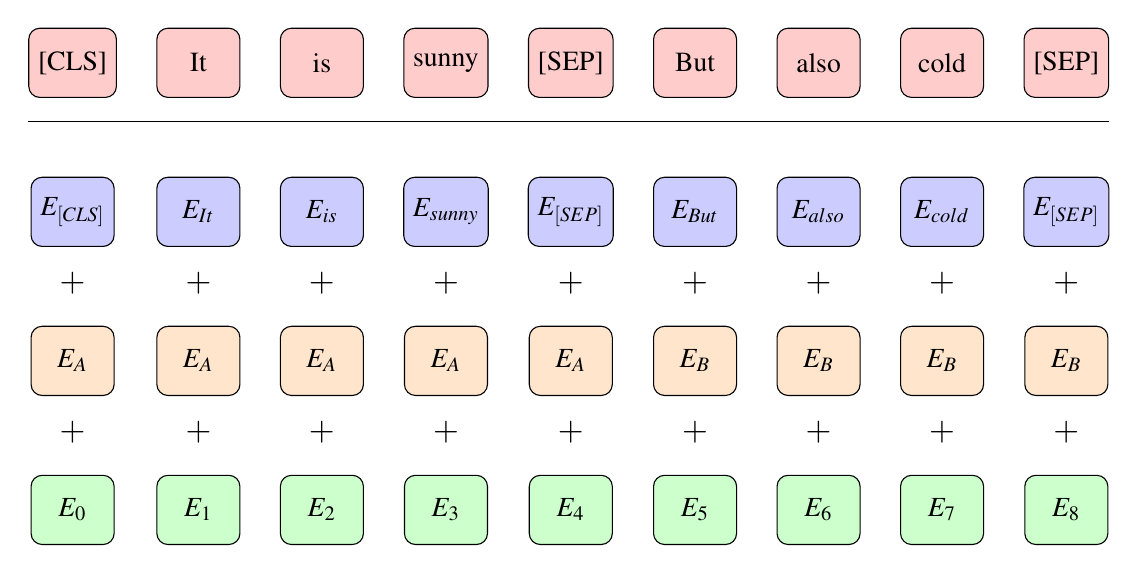
\begin{tikzpicture}[
  input/.style={rectangle, rounded corners, minimum height=2.5em, minimum width=3em, draw, fill=red!20},
  token/.style={rectangle, rounded corners, minimum height=2.5em, minimum width=3em, draw, fill=blue!20},
  seg_embed/.style={rectangle, rounded corners, minimum height=2.5em, minimum width=3em, draw, fill=orange!20},
  pos_embed/.style={rectangle, rounded corners, minimum height=2.5em, minimum width=3em, draw, fill=green!20},
  input_embed/.style={rectangle, rounded corners, minimum height=2.5em, minimum width=3em, draw, fill=purple!20},
  plus/.style={}
]

    % Tokens
    \node[input] (i1) {[CLS]};
    \node[input, right=0.5cm of i1] (i2) {It};
    \node[input, right=0.5cm of i2] (i3) {is};
    \node[input, right=0.5cm of i3] (i4) {sunny};
    \node[input, right=0.5cm of i4] (i5) {[SEP]};
    \node[input, right=0.5cm of i5] (i6) {But};
    \node[input, right=0.5cm of i6] (i7) {also};
    \node[input, right=0.5cm of i7] (i8) {cold};
    \node[input, right=0.5cm of i8] (i9) {[SEP]};

        % Tokens
    \node[token, below=1cm of i1] (t1) {$E_{[CLS]}$};
    \node[token, below=1cm of i2] (t2) {$E_{It}$};
    \node[token, below=1cm of i3] (t3) {$E_{is}$};
    \node[token, below=1cm of i4] (t4) {$E_{sunny}$};
    \node[token, below=1cm of i5] (t5) {$E_{[SEP]}$};
    \node[token, below=1cm of i6] (t6) {$E_{But}$};
    \node[token, below=1cm of i7] (t7) {$E_{also}$};
    \node[token, below=1cm of i8] (t8) {$E_{cold}$};
    \node[token, below=1cm of i9] (t9) {$E_{[SEP]}$};

    % Add plus nodes between inputs
    \draw ($(i1.south west) + (0,-0.3)$) -- ($(i9.south east) + (0,-0.3)$);

        % Segmentation embeddings
    \node[seg_embed, below=1cm of t1] (s1) {$E_{A}$};
    \node[seg_embed, below=1cm of t2] (s2) {$E_{A}$};
    \node[seg_embed, below=1cm of t3] (s3) {$E_{A}$};
    \node[seg_embed, below=1cm of t4] (s4) {$E_{A}$};
    \node[seg_embed, below=1cm of t5] (s5) {$E_{A}$};
    \node[seg_embed, below=1cm of t6] (s6) {$E_{B}$};
    \node[seg_embed, below=1cm of t7] (s7) {$E_{B}$};
    \node[seg_embed, below=1cm of t8] (s8) {$E_{B}$};
    \node[seg_embed, below=1cm of t9] (s9) {$E_{B}$};

    % Position embeddings
    \node[pos_embed, below=1cm of s1] (p1) {$E_{0}$};
    \node[pos_embed, below=1cm of s2] (p2) {$E_{1}$};
    \node[pos_embed, below=1cm of s3] (p3) {$E_{2}$};
    \node[pos_embed, below=1cm of s4] (p4) {$E_{3}$};
    \node[pos_embed, below=1cm of s5] (p5) {$E_{4}$};
    \node[pos_embed, below=1cm of s6] (p6) {$E_{5}$};
    \node[pos_embed, below=1cm of s7] (p7) {$E_{6}$};
    \node[pos_embed, below=1cm of s8] (p8) {$E_{7}$};
    \node[pos_embed, below=1cm of s9] (p9) {$E_{8}$};

    % Pluses at 0.25 between each (s, t) pair
    \node[above=0.25cm of $(s1)!.25!(t1)$, font=\large] {$+$};
    \node[above=0.25cm of $(s2)!.25!(t2)$, font=\large] {$+$};
    \node[above=0.25cm of $(s3)!.25!(t3)$, font=\large] {$+$};
    \node[above=0.25cm of $(s4)!.25!(t4)$, font=\large] {$+$};
    \node[above=0.25cm of $(s5)!.25!(t5)$, font=\large] {$+$};
    \node[above=0.25cm of $(s6)!.25!(t6)$, font=\large] {$+$};
    \node[above=0.25cm of $(s7)!.25!(t7)$, font=\large] {$+$};
    \node[above=0.25cm of $(s8)!.25!(t8)$, font=\large] {$+$};
    \node[above=0.25cm of $(s9)!.25!(t9)$, font=\large] {$+$};


    % Pluses at 0.25 between each (p, s) pair
    \node[above=0.25cm of $(p1)!.25!(s1)$, font=\large] {$+$};
    \node[above=0.25cm of $(p2)!.25!(s2)$, font=\large] {$+$};
    \node[above=0.25cm of $(p3)!.25!(s3)$, font=\large] {$+$};
    \node[above=0.25cm of $(p4)!.25!(s4)$, font=\large] {$+$};
    \node[above=0.25cm of $(p5)!.25!(s5)$, font=\large] {$+$};
    \node[above=0.25cm of $(p6)!.25!(s6)$, font=\large] {$+$};
    \node[above=0.25cm of $(p7)!.25!(s7)$, font=\large] {$+$};
    \node[above=0.25cm of $(p8)!.25!(s8)$, font=\large] {$+$};
    \node[above=0.25cm of $(p9)!.25!(s9)$, font=\large] {$+$};

\end{tikzpicture}
    \caption{BERT: Input Embeddings}
    \label{fig:bert_input}
\end{figure}

\subsection{Text Summarisation}\label{subsec:text-summarisation}
Text summarisation is the task of transforming a piece of text into a shorter  version that retains the most important information.
There are two overarching categories: extractive and abstractive text summarisation.
The former formulates the problem as a subset selection problem by returning only the most salient text excerpts from the original document (\cite{zhong-etal-2020-extractive}), while the latter aims to generate content anew, similar to how humans would do.

We will outline some key models that inspired our work below:
\begin{itemize}
    \item \textbf{Gokhan}: The authors employ an unsupervised summariser based on K-Means clustering of sentences encoded with SentenceBERT (\cite{reimers2019sentence}).
    However, their embeddings are pre-trained on general text, and they suggest that employing in-domain language models would result in a better performance.

    \item \textbf{AMUSE} (\cite{litvak-vanetik-2021-summarization}): The authors design an ETS system comprised of the following steps \begin{enumerate*}
        \item shortening of report with an existing Genetic Algorithm~\cite{litvak-last-2013-multilingual},
        \item encoding sentences with BERT vectors, and
        \item performing binary classification with LSTMs for salient sentence extraction
    \end{enumerate*}.
    They suggest that further work should incorporate \begin{enumerate*}
        \item efficient preliminary sentence removal, and
        \item additional neural modelling stages for the representation and detection of relevant input text parts.
    \end{enumerate*}

    \item \textbf{Hybrid model with RL} (\cite{zmandar-etal-2021-joint}): The authors train a joint extractive-abstractive summarisation model with reinforcement learning optimised for the ROUGE-2 F1 metric.
    Their networks are based on attentive LSTMs augmented with an additional copy mechanism (\cite{vinyals2015pointer}) achieving the second highest F1 score in the FNS21 competition.

    \item \textbf{T5} Hybrid (\cite{orzhenovskii-2021-t5}): The author used T5 (\cite{rayson2019t5}) for a hybrid model fine-tuned to generate the beginning of an abstractive summary and find the closest match of the output in the report’s full text.
    This is the best performing algorithm in the FNS21 competition but also the first to consider transformer models from an abstractive summarisation perspective in the FNP workshops so far.

\end{itemize}

In this work we will be solely exploring the extractive method, and more specifically - the \emph{supervised neural-based} (i.e., RNN, Transformer) type and the \emph{unsupervised graph-based} (i.e., TextRank, LexRank) type.


\subsection{LexRank}\label{subsec:lexrank}
LexRank (\cite{Erkan2004LexRankGC}) is an unsupervised extractive summarisation method consistently used as a baseline in the FNS21 and previous challenges.
It retrieves the most salient document sentences by computing their importance based on \emph{eigenvector centrality}.
To do that the algorithm creates a graph where each sentence represents a node and each edge is a weight between two nodes (\cite{Shearing2020AutomatedTS}).
The sentences are encoded as bag-of-words vectors of size $N$ - the vocabulary size, and the weight metric is a combination of tf-idf (Eq.\ref{eq:idf},\ref{eq:tfidf}) and cosine similarity - Eq.\ref{eq:cosinesimtfidf}.

\begin{equation}
    \text{idf}(t, D) = \log \frac{|D|}{|\{d \in D : t \in d\}|} \label{eq:idf}
\end{equation}

\begin{equation}
    \text{tf-idf}(t, d, D) = \text{tf}(t, d) \cdot \text{idf}(t, D)
    \label{eq:tfidf}
\end{equation}

\begin{equation}
    \text{tf\_idf\_cosine\_similarity}(s_1, s_2) = \frac{\sum_{t \in T} \text{tf-idf}(t, s_1, D) \cdot \text{tf-idf}(t, s_2, D)}{ \sqrt{\sum_{t \in T} \text{tf-idf}(t, s_1, D)^2} \cdot \sqrt{\sum_{t \in T} \text{tf-idf}(t, s_2, D)^2}}
    \label{eq:cosinesimtfidf}
\end{equation}

where $t$ is a term, $d$ is a document within a collection of documents/sentences $D$.

Also, $s_1$ and $s_2$ are two sentences and $T$ represents the set of all terms in both of them while $tf(t, d)$ denotes the term frequency of $t$ in $d$, and $idf(t, D)$ is the inverse document frequency of $t$ in the collection $D$.

The authors further propose finding the most important sentences by \begin{enumerate*}
    \item applying a threshold for the creation of edges with Eq.\ref{eq:cosinesimtfidf},
    \item building an adjacency matrix and normalizing it to produce \emph{transition probabilities},
    \item computing in an iterative fashion the \emph{eigenvector centrality} until convergence, and finally
    \item ranking sentences based on their \emph{lexical} PageRank (\cite{page1998anatomy}) score.
\end{enumerate*}
\section{Methodology}\label{sec:methodology}

\subsection{Data}\label{subsec:data}
The data for the FNS21 task is a collection of narrative parts of annual reports, converted from PDF to plain text.
As discussed in Section~\ref{subsec:fns} due to the rich visual representations in the PDFs, the resulting text suffers from various problems like
\begin{enumerate*}
    \item \emph{spacing inconsistencies} - mixing of tab-space word delimiters, over-segmentation (i.e., a split into incoherent chunks) and under-segmentation (i.e., merging of unrelated words),
    \item \emph{symbol encoding issues} - introduction of unreadable non-alphanumeric characters, and
    \item \emph{formatting issues} - words having different casing, hyphenation at the end of a line, etc
    \item \emph{conversion of tables to text} - financial figures spanning over multiple lines and being mixed with the text.
\end{enumerate*} (Figure~\ref{fig:pdf_to_text}).

% PDF-to-text conversion issues
\begin{figure}[ht]
    \centering
    \begin{enumerate}
        \item \begin{verbatim}
         Following my appointment as Chief
        E x e c u t i v e	in	J u l y	2 0 1 0 ,	g r e ate r	e m p h a s i s
        h a s	b e e n	p l a c e d	o n	f u l fi l l in g	t h e	s u p p l y	o f
        tonnage due under legacy contracts and
    \end{verbatim}
    \item \begin{verbatim}
        However,   the   Directors   further   believe   that   additional
        capital   	could   	be	  deployed	  to 	beneficial   	effect.
    \end{verbatim}
    \item \begin{verbatim}
        Opening net book amount 116,635 35,624 166,754 319,013
        Additions 51,380 7,647 307,546 366,573
    \end{verbatim}
    \item \begin{verbatim}
          This means that buyers can
        _0_@uk_ar06_front.indd   5 20/04/2007   09:13:30 05
        @UK PLC
        Annual Report and Accounts 2006
        use our network to purchase from their suppliers.
    \end{verbatim}
    \end{enumerate}
    \caption{PDF-to-text conversion issues.}
    \label{fig:pdf_to_text}
\end{figure}

To address these issues, we have developed a rigorous data cleaning pipeline that achieves the following key objectives:
\begin{enumerate*}
    \item handles space-tab mixing via hand-crafted rules (derived from observation\footnote{
      E.g., for some of the lines, characters were separated by spaces and words with tabs, hence the need for a custom rule.
    }),
    \item retains alphanumeric characters, punctuation, spaces, financial symbols, and
    \item removes sentences shorter than 3 words
\end{enumerate*}.

As discussed in Section~\ref{subsec:fns}, the annual reports are extremely long documents with an average length reported at 80 pages (\cite{litvak-vanetik-2021-summarization}).
Each one has at least two--three gold summaries provided by the FNS21 organisers, and we compute some statistics
\begin{enumerate*}
    \item helpful for grasping the nature of the output text, but also
    \item useful for the evaluation of the summarisation models
\end{enumerate*}.
On one hand, we can see that the average number of words in the longest summary is over $2,000$ (Figure~\ref{fig:longest_summary_word_count}), while the FNS21 regulations specify an expected output of at most $1,000$ words.
Furthermore, as we are not competing in the FNS21 task, for simplicity, during evaluation we will generate only summaries with at most 40 sentences.
We arrive at this number by observing that the median number of words in the longest summaries is 25 (Figure~\ref{fig:sentence_word_count}), and calculating that $\frac{1,000\text{words}}{25\text{words}}=40$ sentences can suffice.

\begin{figure}[ht]
    \begin{subfigure}{0.49\textwidth}
        \centering        \includegraphics[width=1\columnwidth]{../charts/longest_summary_word_count}
        \caption{Number of words in longest report summary}
        \label{fig:longest_summary_word_count}
    \end{subfigure}%
    \hfill
    \begin{subfigure}{0.49\textwidth}
        \centering
        \includegraphics[width=1\columnwidth]{../charts/sentence_word_count}
        \caption{Number of words in training sentences}
        \label{fig:sentence_word_count}
    \end{subfigure}
    \caption{Distribution of number of words in training sentences and report summaries}
    \label{fig:word_count}
\end{figure}

As we were only provided with the training and the validation FNS21 datasets (Table~\ref{tab:fns21-data}),
we decided to treat the validation set as a testing set (Table~\ref{tab:fns21-my-data})\footnote{
    We observed that two of the annual report files were empty, hence the difference of 3,361 and 3,363 (Table~\ref{tab:fns21-data} without testing set).
} and perform our own training-validation data split on a sentence level instead due to the significant variation in report lengths (\cite{litvak-vanetik-2021-summarization}).
\begin{table}[h]
    \centering
    \begin{tabular}{lrr r}
        \hline
        Data Type & Training + Validation & Testing & Total \\
        \midrule
        Report full text & 2,998 & 363 & 3,361 \\
        \bottomrule
    \end{tabular}
    \caption{Training-Validation-Testing Data Split}
    \label{tab:fns21-my-data}
\end{table}
Specifically, we use a 90--10 \emph{stratified split} (i.e., the label distribution is retained in both sets) for training and validation, respectively.
We are aware that a validation and a training sentence can come from the same report, but we claim that this is not problematic for the following reasons:
\begin{enumerate}
    \item Sentences are \emph{de-contextualised} (i.e., without references or dependencies to others, taken out of context) and \emph{shuffled}.
    \item Sentences contain a \emph{great deal of textual noise} due to the PDF-to-text conversion.
    \item Annual reports are \emph{numerous} but also \emph{extremely long} (i.e., containing a lot of sentences).
\end{enumerate}
Therefore, we believe that the training and validation sentences are to a large extent independent, and as for the process of sentence extraction, we refer you to Section~\ref{subsec:sentence_extraction} for an in-depth discussion.

\subsection{Sentence Extraction}\label{subsec:sentence_extraction}
We approach the annual report summarisation problem from a supervised perspective - we cast the task of Extractive Text Summarisation (ETS) as a binary classification problem defined on the sentence level.
More formally, we can describe the annual report as $d=\{s_{1}, s_{2}, \dots, s_{n}\}$, where $d$ is a document, represented in terms of sentences $s_{i}, \  1 \leq i \leq n$ (\cite{liu2019finetuningbert}).

Then, a candidate summary\footnote{
    A candidate summary is generated from a model $m_{i}$ but it is not yet a \emph{best summary}.
} can be $c=\{s_{1}, s_{2}, \dots, s_{k} | s_{i} \in d \}, \ 0 \leq k \leq n$.
We further need to define the \emph{gold summary}, $c^{*}$ for a document $d$.
In the case of the FNS21 task, there are at least two summaries per report, hence we will use the following notation for the set of all gold summaries for each document $C^{*} = \{c^{*}_{1}, c^{*}_{2}, \dots, c^{*}_{p}\}$.
Furthermore, the supervised learning labels are $y_{i} \in \{1,0\}$ for each sentence $s_{i}$ in $d$ if the sentence is or is not in \textbf{\emph{any}} of the gold summaries $c^{*}_{j}$ for that document.
We argue that in order to increase the positive samples (i.e., the summarizing sentences) we should not restrict
ourselves to just one gold summary in the training process unlike~\cite{orzhenovskii-2021-t5}.
Our goal is to achieve better latent feature extraction of summaries through the employment of all existing data, hence using \textbf{\emph{any}} gold summaries.
However, we are aware that this approach is more likely to encounter standard ETS issues, specifically - extracted summary sentences could be retrieved from unrelated paragraphs in the report.
This can cause the \enquote{dangling anaphora} phenomenon, i.e.\ de-contextualised extracts are stitched together and can mislead the reader due to out-of-context references (\cite{lin2009summarization}).

While some authors (\cite{zmandar-etal-2021-joint}) follow the greedy ROUGE-maximisation method of matching summary
sentences to document sentences (established in~\cite{nallapati2017summarunner}), we approach the problem in a
more practical and faster fashion.
After manual observation of the reports against their gold summaries, it became clear that almost for all sentences
belonging to $c^{*}_{i}$, there was an exact match with a sentence in the whole annual report $d$.

This hypothesis was proven correct by one of the FNS21 contestants (\cite{orzhenovskii-2021-t5}) who reported that
99.4\% of the summaries were included in the report as whole subsequences.
Hence, after having pre-processed the text documents we iteratively match the sentences and generate the binary
classification labels ($\{1,0\}$ representing \emph{summary} and \emph{non-summary}, respectively) for both
the training and testing datasets.

\section{Recurrent Extractor Model}\label{sec:rnn_model}
As our main recurrent model we propose a GRU-based architecture (\cite{cho-etal-2014-learning}), inspired by~\cite{zmandar-etal-2021-joint} and depicted in Figure~\ref{fig:rnn_model}. \\

\begin{minipage}[ht]{0.5\textwidth}
    The model consists of a word embedding layer, a fully-connected feed-forward neural network (FCFFNN), two bidirectional gated recurrent units (GRU) layers, a dot-product attention layer, and a linear projection layer with softmax activation.

    The word embedding layer is used to convert the pre-processed input sentence into a vector representation.
    One of our implementation innovations is that we use FinText's FastText word embeddings~\cite{rahimikia2021realised} because they
    \begin{enumerate*}
        \item are character-based and thus can handle noisy or out-of-vocabulary words, and
        \item are pre-trained on large corpora of financial news, achieving considerable in-domain performance improvements over general-purpose embeddings
    \end{enumerate*}.

    We use the FCFFNN layer to \emph{map the vectorized sentences to a higher-level representation} (similar to~\cite{saikh2020deep}) capturing more complex features or patterns from the input text, but also to \emph{reduce the dimensionality} of the input.

    Two stacked GRU layers are used to \emph{extract the latent recurrent features} from the compressed vector representation in both directions - forward and backward (refer to Section~\ref{subsec:rnn} for details).
\end{minipage}\hfill
\noindent\begin{minipage}[ht]{0.4\textwidth}
    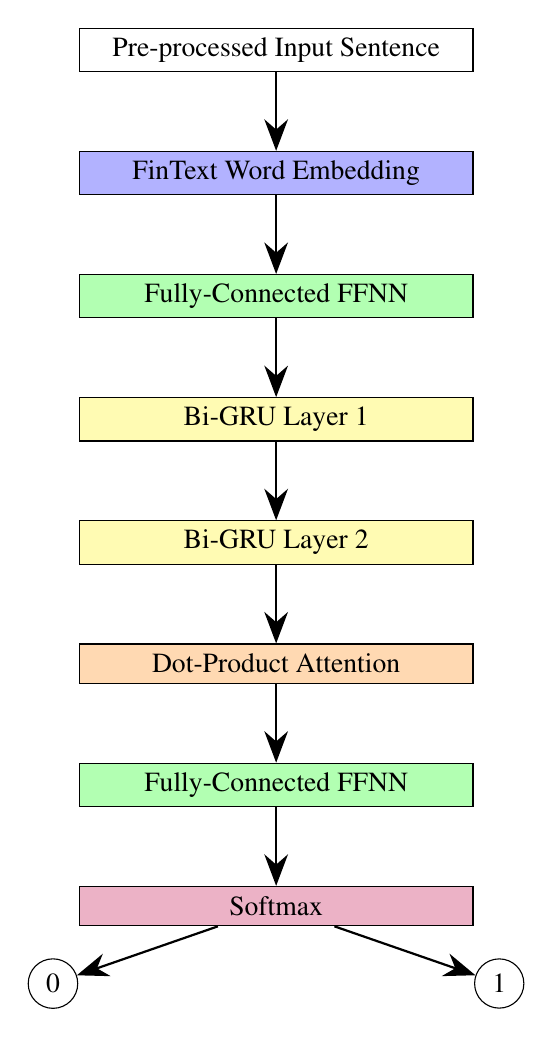
\begin{tikzpicture} [node distance = 0cm and 1cm,    box/.style={draw, rectangle, minimum height=0.5cm, minimum width=5cm},    arrow/.style={-{Stealth[length=4mm]}, thick, font=\footnotesize}]
        % Nodes
        \node[box] (input) {Pre-processed Input Sentence};
        \node[box, fill=blue!30, below=1cm of input] (we) {FinText Word Embedding};
        \node[box, fill=green!30, below=1cm of we] (fc) {Fully-Connected FFNN};
        \node[box, fill=yellow!30, below=1cm of fc] (biGRU1) {Bi-GRU Layer 1};
        \node[box, fill=yellow!30, below=1cm of biGRU1] (biGRU2) {Bi-GRU Layer 2};
        \node[box, fill=orange!30, below=1cm of biGRU2] (dpa) {Dot-Product Attention};
        \node[box, fill=green!30, below=1cm of dpa] (fc2) {Fully-Connected FFNN};
        \node[box, fill=purple!30, below=1cm of fc2] (sf) {Softmax};
        \node[circle, fill=white, draw=black, below left=0.5cm and 0.1cm of sf, minimum size=0.5cm] (bo1) {0};
        \node[circle, fill=white, draw=black, below right=0.5cm and 0.1cm of sf, minimum size=0.5cm] (bo2) {1};

        % Arrows
        \draw[arrow] (input) -- node[right] {} (we);
        \draw[arrow] (we) -- node[right] {} (fc);
        \draw[arrow] (fc) -- node[right] {} (biGRU1);
        \draw[arrow] (biGRU1) -- node[right] {} (biGRU2);
        \draw[arrow] (biGRU2) -- node[right] {} (dpa);
        \draw[arrow] (dpa) -- node[right] {} (fc2);
        \draw[arrow] (fc2) -- node[right] {} (sf);
        \draw[arrow] (sf) -- node[right] {} (bo1);
        \draw[arrow] (sf) -- node[right] {} (bo2);
    \end{tikzpicture}
    \captionof{figure}{GRU-based extractive model}
    \label{fig:rnn_model}
\end{minipage}\\

We further implement the scaled dot-product attention (Eq.\ref{eq:attention_score} from~\cite{vaswani2017attention}) to
compute a new weighted context-aware representation from the extracted features by the GRU layers.

The final layer is a fully-connected feed-forward neural network (FCFFNN) with a softmax activation function, which is
used to \emph{map the latent features to a binary classification} of the input sentence.

\subsection{Hyperparameter Tuning}\label{subsec:hyperparameters}
We have experimented with a number of hyperparameters for our recurrent model, including the use of a FCFFNN,
the recurrence type, the effect of applying attention, the dropout rate, the learning rate, and the effect of data augmentation.

For the analysis we will be extensively using the test accuracy, $F1$-score, and the \emph{summary recall} metric.
The latter is defined as the ratio of the number of correctly predicted summary sentences to the total number of summary sentences in the test dataset.
We consider this metric to be extremely relevant because in the context of extractive summarisation, our goal is to minimise the Type II error (i.e., the number of sentences that should be in the summary but are not).
Our reasoning is that our classifier must be as good as possible in recognising salient sentences (i.e., summarising sentences) even if it introduces some false positives (i.e., non-summarising sentences).
In practice, the user can always remove irrelevant sentences, but it is much harder to add sentences that should have already been in the summary.

Each sentence in the report is represented as a (100, 300)-sized word embeddings vector, where 100 is the longest possible sentence length (i.e., implying long sentences are trimmed) and 300 is the dimensionality of the word embeddings.
We test the effect of inserting an FCFFNN layer between the word embeddings and the GRU layers (each with 64 hidden units) and arrive at the following conclusions:
Adding an FCFFNN layer increases Summary Recall by 2.5\% (Fig.~\ref{fig:summary_recall_FFNN_effect}), but marginally reduces Test Accuracy by less than 1\% (Fig.~\ref{fig:test_accuracy_FFNN_effect}).
We attribute the increase in Summary Recall to the fact that the FCFFNN layer is able to extract an additional mix of features from the word embeddings, which are then used by the GRU layers to make better predictions.
As for the Test Accuracy, we believe that the small decrease is insignificant and we therefore choose to use the FCFFNN layer in our final model.

\begin{figure}[ht]
    \begin{subfigure}{0.49\textwidth}
        \centering \includegraphics[width=1\columnwidth]{../charts/summary_recall_FFNN_effect}
        \caption{Effect of FCFFNN layer on summary recall}
        \label{fig:summary_recall_FFNN_effect}
    \end{subfigure}%
    \hfill
    \begin{subfigure}{0.49\textwidth}
        \centering
        \includegraphics[width=1\columnwidth]{../charts/test_accuracy_FFNN_effect}
        \caption{Effect of FCFFNN layer on test accuracy}
        \label{fig:test_accuracy_FFNN_effect}
    \end{subfigure}
    \caption{Effect of FCFFNN layer on summary precision and test accuracy}
    \label{fig:FCFFNN}
\end{figure}




\begin{enumerate}

\end{enumerate}





\section{Evaluation}\label{sec:evaluation}

To assemble a candidate summary $c_{i}$ we prepare the sentences $s_{j}^{i}$ from a report $d_{m}$ (e.g., embed or tokenize sentences for the GRUs and FinBERT, respectively).
Afterwards, we feed them into our model computing the output summary probabilities $p_{j}^{i}$, and then we select the
top-$k$ sentences ($k=40$, Section~\ref{subsec:data}) based on the highest sentence probabilities $p_{j}^{i}$.
Finally, we concatenate them to form the summary $c_{i}$ in natural order (i.e., the order in the input text),
but also trim it to the maximum length of $1,000$ words (Section~\ref{subsec:fns}).

In general, to assess the quality of a candidate summary $c$, we measure its similarity with the gold summary $c^{*}$
based on their n-gram overlap $R=(c, c^{*})$, where $R$ is the ROUGE-$F_{1}$\footnote{
    \begin{itemize}
        \item We use a slightly different but faster version of ROUGE compared to the official metric~\cite{lin2004rouge}.
              It can be accessed at: \url{https://github.com/pltrdy/rouge}
        \item The FNS21 evaluation metric is the $F1$-score of ROUGE-2, and we will use it for the final evaluation.
    \end{itemize}
} metric(\cite{lin2004rouge}).
For the FNS21 task due to the extractive nature of our approach we will evaluate our models based on
the ROUGE-L--maximising $c^{*}_{i}$ gold summary (Section~\ref{subsubsec:rouge}), i.e.,

\begin{figure}[h]
    \centering
    \begin{equation}\label{eq:rouge_max}
        r = \underset{c^{*} \in C^{*}}{\operatorname{argmax}} R(c, c^{*}_{i})
    \end{equation}
    \caption{Candidate summary evaluation as a gold summary ROUGE-maximisation}
    \label{fig:rouge_max}
\end{figure}

The intuition is that by extracting multiple sentences from the report, our generated candidate summary can
retain sentences from \emph{any} of the gold summaries.
Hence, there must be at least one such gold summary where the longest common subsequence overlap (ROUGE-L) is maximal.
The practical implications are that two models, $m_{1}$ and $m_{2}$ can produce two different candidate summaries
$c_{1}$ and $c_{2}$, respectively.
Their individual evaluation is based on gold summaries $c^{*}_{1}$ and $c^{*}_{2}$ (which can be the same when the
candidates $c_{1}$ and $c_{2}$ are identical).
This guarantees that we are always comparing candidate summaries based on their maximal evaluation scores.

Following this evaluation mechanism, we compare our models in terms of their ROUGE metrics in Table~\ref{tab:rouge_performance}.
Please keep in mind that we include official results from the FNS21 competition for comparison, namely the T5-LONG-EXTRACT model
(\cite{orzhenovskii-2021-t5}) and the MUSE model (\cite{litvak-last-2013-multilingual}), which have been
\begin{enumerate*}
    \item trained on more data than our models due to us using the official validation as a test set (see Section~\ref{subsec:data}),
    \item evaluated on the official test set which we did not have access to
\end{enumerate*}.

\begin{table}[ht]
    \centering
    \begin{tabular}{lccc}
        \toprule
        \textbf{Model} & \textbf{ROUGE-1} & \textbf{ROUGE-2} & \textbf{ROUGE-L} \\
        \midrule
            $\star$ FinBERT-base & 0.544 & 0.382 & 0.524 \\
            T5-LONG-EXTRACT (\cite{orzhenovskii-2021-t5})* & 0.54 & 0.38 & 0.52 \\
            FinBERT-base + back-translation & 0.490 & 0.321 & 0.468 \\
            MUSE (\cite{litvak-last-2013-multilingual})* & 0.5 & 0.28 & 0.45 \\
            $\star$ GRU-base + attention + back-translation & 0.276 & 0.106 & 0.249 \\
            GRU-base + back-translation & 0.266 & 0.100 & 0.247 \\
            LexRank & 0.250 & 0.086 & 0.227 \\
            TaxtRank & 0.220 & 0.064 & 0.196 \\
            GRU-base & 0.220 & 0.063 & 0.201 \\
            GRU-base + attention & 0.221 & 0.062 & 0.204 \\
        \bottomrule
    \end{tabular}\caption{ROUGE: Model performance on the FNS21 test dataset.}
    \label{tab:rouge_performance}
\end{table}

We can provide the following commentary on the results:
\begin{itemize}
    \item The best performing model is FinBERT-base (\cite{yang2020finbert}), which is a pre-trained on financial communication documents,
        achieving a ROUGE-2 score of $0.382$, which is \emph{at least as good as the official best-performing model} in the FNS21 competition:
        the T5-LONG-EXTRACT (\cite{orzhenovskii-2021-t5}, Section~\ref{subsec:text-summarisation}).
        Surprisingly, data augmentation does not improve the performance of FinBERT-base, and we believe this was caused by
        the \hyperlink{data_augment_hypothesis}{back-translation hypothesis} we made in Section~\ref{subsec:hyperparameters}.
        Nevertheless, both models outperform the official top-line (\cite{litvak-last-2013-multilingual}) by a significant margin for ROUGE-2.
    \item The GRU-base + attention + back-translation model is the best performing model out of all recurrent neural architectures.
    While preliminary binary classification results did not show any considerable differences between the models, clearly
    \begin{enumerate*}
        \item the attention mechanism helps the model to better recognise the summarising sentences (i.e., attends to the most descriptive linguistic features), and
        \item the back-translation data augmentation significantly improves the practical performance of the model (i.e., the probability distribution of the summarising sentences).
    \end{enumerate*}
    \item At the same time, we acknowledge that the universal summarisation baselines: LexRank and TextRank, outperform
        our simple GRU models, and we attribute this to both:
    \begin{enumerate*}
        \item the lack of sufficient descriptive training data from the positive class (i.e., the summarising sentences, Table~\ref{tab:random_under_sampling}),
        \item the 90\% random under-sampling of the majority class data (see Section~\ref{subsec:data}), and
        \item the summary generation process of selecting the top $k$ sentences based on their sorted probabilities (see discussion in Sections~\ref{subsec:qualitative-discussion} and~\ref{subsec:limitations}).
    \end{enumerate*}
\end{itemize}

\subsection{Qualitative Discussion}\label{subsec:qualitative-discussion}
After having established the quantitative performance of our models, we now turn to the qualitative discussion of the results.
For a random annual report we generated a summary using the FinBERT-base + data augmentation model and
the GRU-base + attention model (see Figure~\ref{fig:summary_examples}
where green colour indicates the summarising sentences, and red colour -- the non-summarising sentences).
We can make the following conclusions based on observation:
\begin{enumerate}
    \item The FinBERT-base model has \emph{around 50\% of its contents} belonging to any of the gold summaries (Figure~\ref{fig:finbert_summary}),
        while all other sentences look very convincing in terms of their summarising potential (i.e., they are informative of the financial situation but also concise)
    \item At the same time, the GRU-model has the opposite characteristics:
    \begin{enumerate*}
        \item none of its sentences are in the gold summary (Figure~\ref{fig:rnn_summary}), while
        \item all of them are very long, containing uninformative but diverse sets of words, which in turn results in higher ROUGE scores.
    \end{enumerate*}.
    This clearly represents the problem of using ROUGE as a metric for summarisation since it is only measures the lexical overlap, while being semantically unaware (\cite{akter-etal-2022-revisiting}).
\end{enumerate}
While we acknowledge that the GRU model seems to be biased towards long and noisy sentences, we must note that in the example
only $5$ sentences have been generated to fit the word limit.
As we demonstrated that our model is accurate at recognising the summarising sentences (Section~\ref{subsec:hyperparameters}),
we believe that it is more of a summary generation issue (i.e., the mechanism to combine predicted sentences into a single summary)
rather than a classification issue (see Section~\ref{subsec:limitations}).

Although, the practical results from Figure~\ref{fig:summary_examples} might seem disappointing, we must once again remind the reader that the reports are extremely
long with an average number of sentences and words at around $2,700$ and $58,000$, respectively (\cite{litvak-vanetik-2021-summarization}).
Meanwhile, we are constrained to producing a summary of at most $40$ sentences (Section~\ref{subsec:data}) or $1,000$ words (Section~\ref{subsec:fns}).

\begin{figure}[ht]
    \centering
    \begin{subfigure}[t]{0.49\textwidth}
        \centering
        \includegraphics[width=\textwidth]{../charts/transformer-example-summary}
        \caption{Example summary from the FinBERT-base + data augmentation model.}
        \label{fig:finbert_summary}
    \end{subfigure}
    \hfill
    \begin{subfigure}[t]{0.49\textwidth}
        \centering
        \includegraphics[width=\textwidth]{../charts/rnn_summary}
        \caption{Example summary from the GRU-base + attention model.}
        \label{fig:rnn_summary}
    \end{subfigure}
    \caption{Examples of summaries produced by our models.}
    \label{fig:summary_examples}
\end{figure}


\section{Conclusion}\label{sec:conclusion}
\subsection{Summary of Achievements}\label{subsec:summary}
In this project we have explored the problem of summarising UK annual reports.
To deal with the significant amount of noise in the plain text of these glossy documents, we have built a rigorous pre-processing pipeline (Section~\ref{subsec:data}).
We have further implemented a sentence extraction phase where we generate binary labels ($1$ being summary, $0$ - non-summary) from the reports and their multiple gold summaries (Section~\ref{subsec:sentence_extraction}).
Once our datasets are created, we
\begin{enumerate*}
    \item design a Recurrent Neural Network (RNN) architecture (Section~\ref{subsec:rnn_model}), and
    \item fine-tune a financial Transformer model - FinBERT (Section~\ref{subsec:finbert})
\end{enumerate*},
training them in a supervised manner for a binary classification task (Sections~\ref{subsec:training} and~\ref{subsec:hyperparameters}).
We quantitatively evaluate our models with the ROUGE metric and demonstrate them outperforming traditional baselines (Section~\ref{sec:evaluation}).
Furthermore, at least for FinBERT we observe a clear ROUGE-2 improvement over an official FNS21 topline but also a
competitive performance with the best FNS21 extractive model, although noting that the our models are tested on different data (Section~\ref{subsec:data}).
We also discuss the quality of the produced summaries (Section~\ref{subsec:qualitative-discussion}), and in
Section~\ref{subsec:limitations} we describe in more depth the limitations of our system and possible solutions.
\\
In terms of \emph{innovational aspects} of our project in the context of the FNS challenge, we are the first to our knowledge that:
\begin{itemize}
    \item \emph{Integrate FinText word embeddings} - While some FNS21 competitors use general-domain sentence embeddings
    based on BERT (\cite{litvak-vanetik-2021-summarization, gokhan-etal-2021-extractive}), we represent sentences as
    a vector of word embeddings purpose-built for financial text analysis (\cite{rahimikia2021realised}).
    \item \emph{Perform back-translation as data augmentation} - In contrast to approaches where only the first 10\% of
    the annual report is used (\cite{orzhenovskii-2021-t5}), we over-sample the summarising sentences (minority class)
    by back-translating from French.
    \item \emph{Fine-tune FinBERT (\cite{yang2020finbert}) for extractive summarisation} - Transformer-based models have become increasingly
    popular in the next edition of the FNP Workshop (FNP22) (\cite{khanna-etal-2022-transformer, pant-chopra-2022-multilingual}),
    where some have used FinBERT for classifying definitions (\cite{ghosh-etal-2022-finrad}),
    detecting hypernyms (\cite{peng-etal-2022-discovering}), and classifying financial sentiments (\cite{stepisnik-perdih-etal-2022-sentiment}).
    However, we are the first to adapt FinBERT for extractive summarisation.
\end{itemize}

\subsection{Discussion of Limitations}\label{subsec:limitations}
Although, both our models have outperformed the baselines on ROUGE-2 and the fine-tuned FinBERT has achieved competitive
performance for the FNS21 task, there are several limitations that we would like to discuss:
\begin{itemize}
    \item \emph{Summary Generation} - In our work we take top $k$ sentences based on the model's output probability distribution (Section~\ref{sec:evaluation}).
        However, this is a very simplistic approach to summarisation that
        \begin{enumerate*}
            \item introduces incoherence issues (like the \emph{dangling anaphora phenomenon} from Section~\ref{subsec:sentence_extraction}),
            \item trims the last sentence to fit the $1,000$ word limit, and it
            \item does not account for the \emph{informativeness} of the individual sentences
        \end{enumerate*}.
        To address the incoherence issues, we can try resolving the correferences in the either through a
        graph-based approach on the generated summary (\cite{sonawane2016coreference}), or by introducing a more complex
        encoder architecture that represents and attends to entities as well as sentences (\cite{Huang2021ExtractiveSC}).
        Regarding the trimming heuristic, a natural improvement can be to use text compression techniques for the final predicted sentence (\cite{ghalandari2022efficient, KNIGHT200291}).
        As for the third point, we believe this is very exacerbating reason why our GRU architecture returns a summary
        without any single whole--sentence overlap with the gold standard (Fig.~\ref{fig:rnn_summary}).
        Instead, what \cite{zmandar-etal-2021-joint} propose is a reinforcement learning approach which incorporates
        the \emph{sentence-level} ROUGE-2 score with the whole gold summary.
        While this method is much more sophisticated, it conveys the intuitive idea that the top-$k$ sentences comprising the
        \emph{optimal candidate summary} should be \emph{greedily maximising the global summary-level ROUGE-2} score.
\end{itemize}

\subsection{Future Work}\label{subsec:future-work}

%\printbibliography %Prints bibliography
\bibliography{refs}             % this causes the references to be
                                % listed

\bibliographystyle{alpha}       % this determines the style in which
                                % the references are printed, other
                                % possible values are plain and abbrv
%% Appendices start here
%\appendix
\section{Appendix}\label{sec:appendix}
\subsection{UK annual report example}\label{subsec:uk-annual-report-example}
\begin{figure}[ht]
    \begin{subfigure}{0.49\textwidth}
        \centering
        \includegraphics[width=1\columnwidth]{../charts/1}
    \end{subfigure}%
    \hfill
    \begin{subfigure}{0.49\textwidth}
        \centering
        \includegraphics[width=1\columnwidth]{../charts/2}
    \end{subfigure}~\caption{Excerpts from Oxfam's 2021--2022 (glossy) annual report}
    \label{fig:oxfam1}
\end{figure}

\begin{figure}[ht]
    \begin{subfigure}{0.49\textwidth}
        \centering
        \includegraphics[width=1\columnwidth]{../charts/3}
    \end{subfigure}%
    \hfill
    \begin{subfigure}{0.49\textwidth}
        \centering
        \includegraphics[width=1\columnwidth]{../charts/4}
    \end{subfigure}~\caption{Excerpts from Oxfam's 2021--2022 (glossy) annual report}
    \label{fig:oxfam2}
\end{figure}

\vfill 

\subsection{Example Model Summaries}\label{subsec:example-model-summaries}
\begin{figure}[ht]
    \centering
    \includegraphics[width=\textwidth]{../charts/transformer-example-summary}
    \caption{Example summary from the FinBERT-base + data augmentation model.}
    \label{fig:finbert_summary}
\end{figure}

\begin{figure}[ht]
        \centering
        \includegraphics[width=\textwidth]{../charts/rnn_summary}
        \caption{Example summary from the GRU-base + attention model.}
        \label{fig:rnn_summary}
\end{figure}

\end{document}
